\subsection{Anotações semânticas}

Reconhecida a importância da web semântica para o acesso e organização de informação. E dada a sua importância para a valorização do conteúdo em motores de busca.\\

Considerou-se essencial para o sucesso do sistema e dos seus utilizadores a utilização de anotações semânticas nas páginas web desenvolvidas.\\

As páginas onde estas anotações mais se justificavam eram na listagem de projetos públicos do sistema, e no perfil de um projeto.

Pretende-se assim que com as referidas anotações, os projetos sejam valorizados nos motores de busca e assim mais facilmente encontrados pelos utilizadores, mas também contribuir para o número de projetos em que o referido autor será associado.\\

Segue-se um gráfico representativo de um excerto da página de procura de projetos públicos:

\begin{figure}[H]
  \centering
  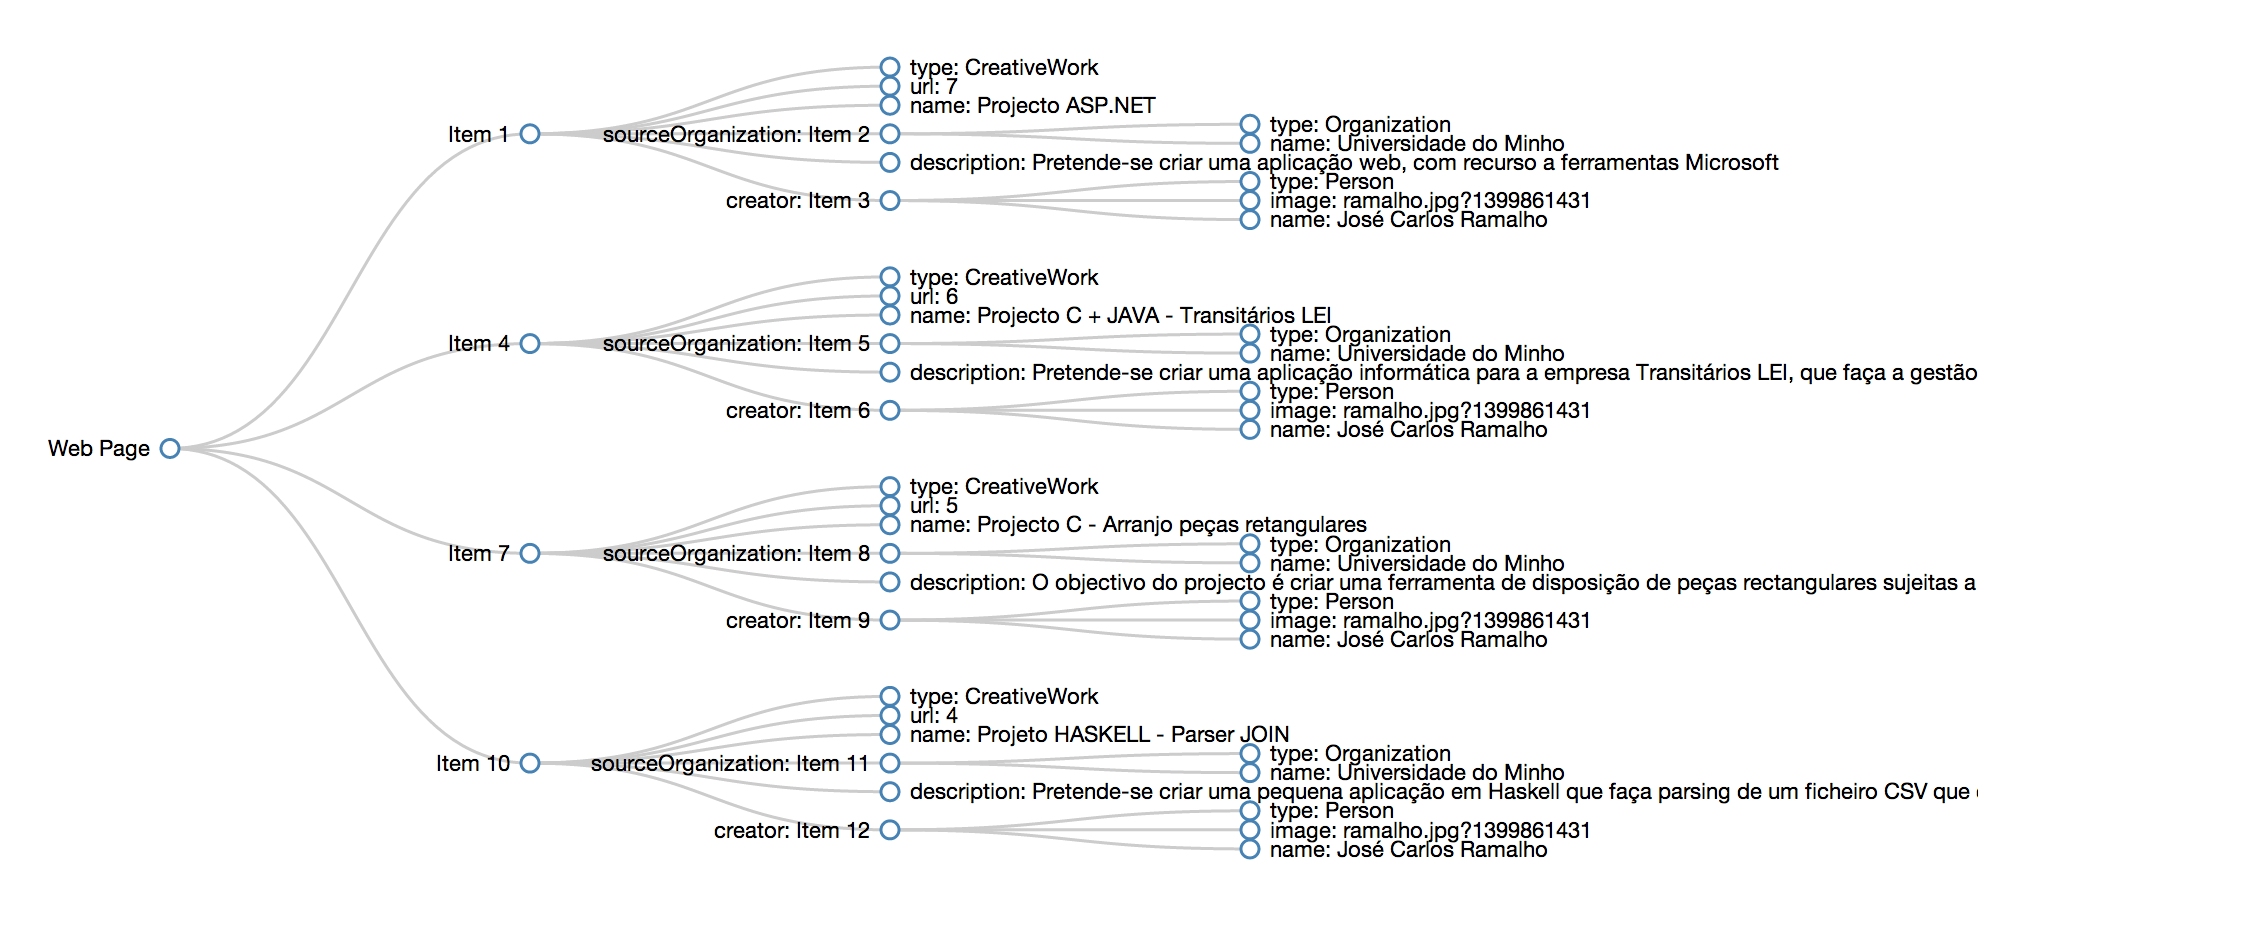
\includegraphics[width=1\textwidth,center]{images/implementacao/rdfa}
  \caption{Anotações semânticas na página de pesquisa de projetos públicos}
\end{figure}

Segue-se a mesma informação representada na forma de dados:
\begin{verbatim}
@prefix rdfa: <http://www.w3.org/ns/rdfa#> .
@prefix schema: <http://schema.org/> .
@prefix rdf: <http://www.w3.org/1999/02/22-rdf-syntax-ns#> .

<http://rdfa.info/play/>
   rdfa:usesVocabulary schema: .
_:1 
   rdf:type schema:CreativeWork;
   schema:url <http://rdfa.info/projects/7>;
   schema:name "Projecto ASP.NET"@en;
   schema:sourceOrganization _:2;
   schema:description "Pretende-se criar uma aplicação web, com recurso a ferramentas Microsoft"@en;
   schema:creator _:3 .
_:2 
   rdf:type schema:Organization;
   schema:name "Universidade do Minho"@en .
_:3 
   rdf:type schema:Person;
   schema:image <http://rdfa.info/system/users/avatars/000/000/001/thumb/ramalho.jpg?1399861431>;
   schema:name "José Carlos Ramalho"@en .
_:4 
   rdf:type schema:CreativeWork;
   schema:url <http://rdfa.info/projects/6>;
   schema:name "Projecto C + JAVA - Transitários LEI"@en;
   schema:sourceOrganization _:5;
   schema:description "Pretende-se criar uma aplicação informática para a empresa Transitários LEI, que faça a gestão de camiões, localidades e clientes."@en;
   schema:creator _:6 .
_:5 
   rdf:type schema:Organization;
   schema:name "Universidade do Minho"@en .
_:6 
   rdf:type schema:Person;
   schema:image <http://rdfa.info/system/users/avatars/000/000/001/thumb/ramalho.jpg?1399861431>;
   schema:name "José Carlos Ramalho"@en .
_:7 
   rdf:type schema:CreativeWork;
   schema:url <http://rdfa.info/projects/5>;
   schema:name "Projecto C - Arranjo peças retangulares"@en;
   schema:sourceOrganization _:8;
   schema:description "O objectivo do projecto é criar uma ferramenta de disposição de peças rectangulares sujeitas a várias restrições que permita ao utilizador colocar as peças na área de trabalho e verificar se todas as restrições são cumpridas. Adicionalmente, deveria ser possível pedir ao sistema para gerar soluções válidas ou mesmo encontrar a melhor solução possível."@en;
   schema:creator _:9 .
_:8 
   rdf:type schema:Organization;
   schema:name "Universidade do Minho"@en .
_:9 
   rdf:type schema:Person;
   schema:image <http://rdfa.info/system/users/avatars/000/000/001/thumb/ramalho.jpg?1399861431>;
   schema:name "José Carlos Ramalho"@en .
_:10 
   rdf:type schema:CreativeWork;
   schema:url <http://rdfa.info/projects/4>;
   schema:name "Projeto HASKELL - Parser JOIN"@en;
   schema:sourceOrganization _:11;
   schema:description "Pretende-se criar uma pequena aplicação em Haskell que faça parsing de um ficheiro CSV que contém as inscrições das JOIN(Jornadas de Informática da Universidade do Minho) e que gere crachas para os diferentes tipos de participantes. A aplicação criada deverá também geras estatísticas sobre as inscrições."@en;
   schema:creator _:12 .
_:11 
   rdf:type schema:Organization;
   schema:name "Universidade do Minho"@en .
_:12 
   rdf:type schema:Person;
   schema:image <http://rdfa.info/system/users/avatars/000/000/001/thumb/ramalho.jpg?1399861431>;
   schema:name "José Carlos Ramalho"@en .
\end{verbatim}

Para a referida anotação semântica, recorreu-se à a \textit{RDFa} e à coleção de \textit{schemas} do \textit{http://schema.org/}.
